\documentclass{article}
\usepackage{amsmath, sfmath, multicol, tkz-euclide, array, enumerate, tcolorbox, tabularray, tipa}
\renewcommand{\familydefault}{\sfdefault}
\setlength{\parindent}{0cm}
\pagestyle{empty}
\usepackage[left=1in, top=0.5in, right=1in, bottom=0.5in]{geometry}
\tikzset{>=stealth, label style/.append style={font=\footnotesize}}
\tcbset{colback=white}

\newcounter{example}[section]
\newenvironment{example}[1][]{\refstepcounter{example}\par\medskip
   {\color{red}\textbf{Example~\theexample. #1}}}{\medskip}

\newcommand{\arc}[1]{%
    \setbox9=\hbox{#1}%
    \ooalign{\resizebox{\wd9}{\height}{\texttoptiebar{\phantom{A}}}\cr#1}}

\begin{document}

\section*{Circles in the Coordinate Plane}

\begin{tcolorbox}[colframe=orange!70!white, coltitle=black, title=\textbf{Today I Can}]
\begin{enumerate}
    \item Write the equation of a circle.
    \item Find the center and radius of a circle.
\end{enumerate}
\end{tcolorbox}
\smallskip 

The equation of a circle with radius $r$ and center ($h$, $k$) is 
\[
(x-h)^2 + (y-k)^2 = r^2
\]
\begin{center}
\begin{tikzpicture}
\draw (-2,0) -- (4,0);
\draw (0,-2) -- (0,4);
\coordinate (B) at (1.5,1.5);
\draw [fill=black] (1.5,1.5) circle (2pt);
\draw (1.5,1.5) circle (2);
\node at (1.5,1.5) [anchor=north] {($h$, $k$)};
\tkzDefShiftPoint[B](40:2){A}
\draw (1.5,1.5) -- (A);
\tkzLabelSegment(A,B){$r$}
\end{tikzpicture}
\end{center}
\bigskip

\begin{example}
Write the equation for each circle.
\begin{enumerate}[(a)]
    \begin{multicols}{2}
        \item Center ($-15$, 1); radius: 2
        \item Center ($-4$, 4); radius: 8 
    \end{multicols}
    \vspace{1.5in}
    \begin{multicols}{2}
        \item Center ($-4$, 8); Point on circle (0, $-10$)
        \item Center (4, 13); Point on circle (0, 16) 
    \end{multicols}
    \vfill 
    \newpage 
    \begin{multicols}{2}
        \item \mbox \newline 
        \item \mbox \newline 
    \end{multicols}    
\end{enumerate}
\begin{minipage}{0.5\textwidth}
    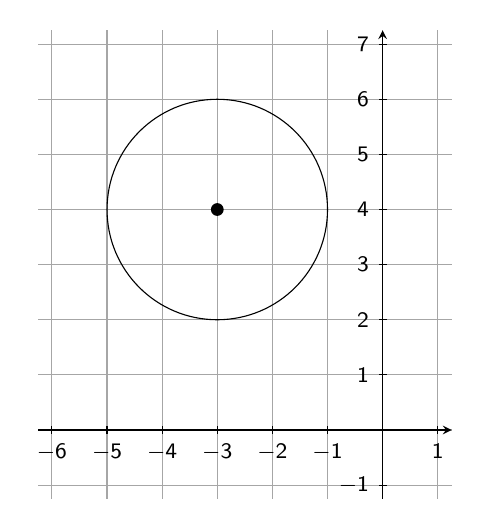
\begin{tikzpicture}[scale=0.7]
    \draw [color=gray!70] (-6.25,-1.25) grid (1.25,7.25);
    \draw[->,color=black] (-6.25,0.) -- (1.25,0.);
    \foreach \x in {-6,-5,-4,-3,-2,-1,1}
    \draw[shift={(\x,0)},color=black] (0pt,2pt) -- (0pt,-2pt) node[below] {\footnotesize $\x$};
    \draw[->,color=black] (0.,-1.25) -- (0.,7.25);
    \foreach \y in {-1,1,2,3,4,5,6,7}
    \draw[shift={(0,\y)},color=black] (2pt,0pt) -- (-2pt,0pt) node[left] {\footnotesize $\y$};
    \draw (-3,4) circle (2cm);
    \draw [fill=black] (-3,4) circle (3pt);
    \end{tikzpicture}
\end{minipage}
\begin{minipage}{0.4\textwidth}
    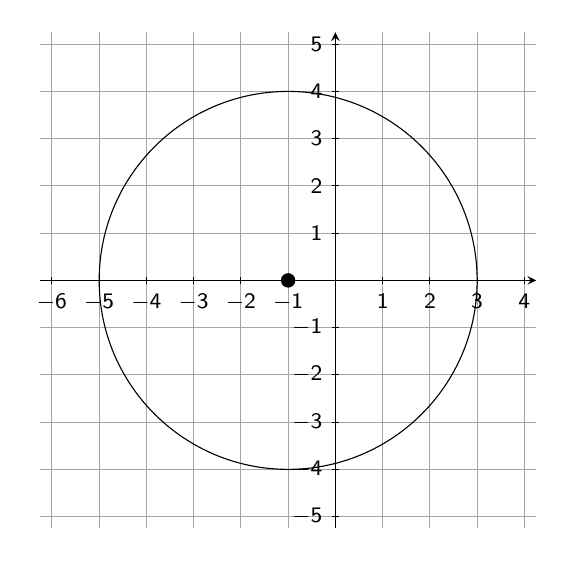
\begin{tikzpicture}[scale=0.6]
    \draw [color=gray!70] (-6.25,-5.25) grid (4.25,5.25);
    \draw[->,color=black] (-6.25,0.) -- (4.25,0.);
    \foreach \x in {-6,-5,-4,-3,-2,-1,1,2,3,4}
    \draw[shift={(\x,0)},color=black] (0pt,2pt) -- (0pt,-2pt) node[below] {\footnotesize $\x$};
    \draw[->,color=black] (0.,-5.25) -- (0.,5.25);
    \foreach \y in {-5,-4,-3,-2,-1,1,2,3,4,5}
    \draw[shift={(0,\y)},color=black] (2pt,0pt) -- (-2pt,0pt) node[left] {\footnotesize $\y$};
    \draw (-1,0) circle (4cm);
    \draw [fill=black] (-1,0) circle (4pt);
    \end{tikzpicture}
\end{minipage}
\end{example}

\vfill 

\begin{example}
Identify the center and radius of each.
\begin{multicols}{2}
\begin{enumerate}[(a)]
    \item $(x+1)^2+(y-8)^2=16$
    \item $(x-6)^2+(y-5)^2=9$
\end{enumerate}
\end{multicols}
\end{example}

\vfill 

\end{document}
